\documentclass[a4paper,twoside,12pt]{memoir}
\usepackage{diplomski}

% Ne znam
\pagestyle{headings}

% Podrška za hrvatski
\usepackage[croatian]{babel}
\usepackage[utf8]{inputenc}
\usepackage[T1]{fontenc}

% Veći razmak između paragrafa
\setlength{\parskip}{\bigskipamount}
% Makni indentaciju na početku paragrafa
\setlength{\parindent}{0pt}
% Dodaj kompaktnije liste
\usepackage{paralist}
% Smanji razmak nakon slika
\setlength{\belowcaptionskip}{-10pt}

% Pretvori linkove u hyperlinkove
\usepackage{hyperref}
% Pretvori URLove u hyperlinkove
\usepackage{url}

% Degree symboli
\usepackage{gensymb}

% Omogući slike
\usepackage{graphicx}
% Omogući popis slika
\usepackage{float}
% Promjeni defaultni folder za slike
\graphicspath{{./images/}}

\title{Pretraživanje}
\author{Janko Marohnić}
\advisor{Prof. dr. sc. Robert Manger}
\date{Travanj, 2015.}

% TODO: Highlighting

\begin{document}

\frontmatter

\chapter{Uvod}

* Quality vs quantity
  - Prouči kako se točno dobiva quality, i što se možda treba žrtvovati
* Uvedi pojam "dokumenta"
* Ako korisnik ne može naći dokument, on "ne postoji"
* Bavimo se isključivo softverima otvorenog koda
* Pojam tražilice (i aplikacije)

Pretraživanje se može opisati u četiri dijela:

\begin{compactenum}
  \item \textbf{Indeksiranje} – Datoteke i baze podataka obrađuju se i pripremaju za pretraživanje
  \item \textbf{Upit} – Korisnik upisuje ključne riječi kroz neku vrstu korisničkog sučelja, i tražilica pronalazi sve dokumente koji odgovaraju upitu
  \item \textbf{Rangiranje} – Tražilica rangira pronađene dokumente s obzirom koliko dobro odgovaraju upitu
  \item \textbf{Prikaz rezultata} – Konačni rezultati se prikazuju u korisničkom sučelju.
\end{compactenum}

\textit{Indeksiranje}, \textit{upit} i \textit{rangiranje} obradit ćemo u sljedećim poglavljima, dok ćemo \textit{prikaz rezultata} izostaviti, jer je to problem isključivo dizajnerske prirode.

\chapter{Indeksiranje} \label{indexing}

Prije nego korisnik napravi bilo kakav upit, tražilica treba "poznavati" sadržaj koji pretražuje. Na primjer, ako dokumenti koji se pretražuju imaju naslov, i mi znamo da je taj naslov puno informativniji od tijela dokumenta, možemo informirati tražilicu da da veću težinu dokumentima kojima je dio upita pronađen u naslovu, time ih rangirajući više u rezultatima.

Nakon što se postiglo određeno razumijevanje dokumenata koji se pretražuju, proces obrade tih dokumenata za pretraživanje, zvan \textit{indeksiranje}, može početi, i opisan je u sljedećim sekcijama. Indeksiranje se vrši prije bilo kojeg upita, zato da onda pri samom upitu tražilica može brzo pronaći i rangirati dokumente.

\section{Preprocesiranje}

Prije samog obrađivanja, potrebno je sve dokumente svesti na jednu zajedničku tekstualnu reprezentaciju. Pretpostavimo da radimo aplikaciju koja omogućuje pohranjivanje digitalnih prezentacija, koje se učitavaju u PDF formatu, i koje se onda mogu gledati online\footnote{Jedna takva aplikacija je \url{http://speakerdeck.com}.}. Htjeli bismo omogućiti da korisnici mogu pretraživati bazu svih prezentacija po ključnim riječima. Problem je što je PDF tzv \textit{binarni} format, pa nije moguće samo pretraživati sadržaj datoteke. Stoga je potrebno danu PDF datoteku najprije svesti na neki format koje je pogodan za pretraživanje. Taj proces pretvaranja više vrsta datoteka u jednu zajedničku tekstualnu reprezentaciju zove se \textit{preprocesiranje}\footnote{\cite{taming} str. 32}.

Neki od češćih formata datoteki su:

\begin{center}
  \begin{tabular}{ll}
    \textbf{Format}                            & \textbf{Esktenzija} \\
    Tekst                                      & .txt                \\
    Microsoft Office (Word, PowerPoint, Excel) & .doc,.ppt,.xls      \\
    Adobe Portable Document Format (PDF)       & .pdf                \\
    Rich Text Format (RTF)                     & .rtf                \\
    HTML                                       & .html               \\
    E-mail                                     & N/A                 \\
    Baze podataka                              & N/A                 \\
  \end{tabular}
\end{center}

Jedan popularan softver otvorenog koda za izdvajanje teksta iz različitih tipova datoteki je Apache Tika\footnote{\url{http://tika.apache.org}}.

\section{Tokenizacija}

Pretraživanje dokumenata svodi se na ispitivanje u kojim se dokumentima pojavljuju ključne riječi unešene u polje za pretraživanje. Svaki dokument se stoga rastavlja na "riječi", tzv \textit{tokene}, tako da se onda pretraživanje dokumenata može ugrubo svesti na traženje ključnih riječi u listi tokena.

Međutim, sama tokenizacija nije tako trivijalan zadatak. Pretpostavimo da trebamo tokenizirati sljedeći tekst:

\begin{quote}
  \textit{Sve današnje skijaške discipline nastale su 1900-1950. godine.}
\end{quote}

Budući da su riječi odvojene razmacima, promotrimo (naivni) tokenizator \textit{A} koji rastavlja tokene po razmacima:

\begin{center}
  \begin{tabular}{|c|c|c|c|c|c|c|c|}
    Sve & današnje & skijaške & discipline & nastale & su & 1900-1950. & godine.
  \end{tabular}
\end{center}

Dok ovaj pristup funkcionira u nekim slučajevima, primijetimo da se kod našeg teksta na zadnji token nalijepila točka, što ne želimo. Promotrimo sada tokenizator \textit{B} koji odstranjuje interpunkcijske znakove:

\begin{center}
  \begin{tabular}{|c|c|c|c|c|c|c|c|}
    Sve & današnje & skijaške & discipline & nastale & su & 1900-1950 & godine
  \end{tabular}
\end{center}

Dok ovaj tokenizator riješava problem lijepljenja interpunkcijskih znakova za tokene, činjenica da su odstranjeni svi interpunkcijski znakovi stvara novi problem. Pretpostavimo da korisnik pretražuje sve dokumente gdje se pojavljuje fraza "pobjednik Ivica Kostelić", i naiđe na sljedeći tekst:

\begin{quote}
  \textit{Prvo mjesto svjetskog skijaškog kupa odnosi novi pobjednik. Ivica Kostelić, nažalost, osvojio je 25. mjesto u prvoj vožnji i nosi porazno zadnje mjesto.}
\end{quote}

Ukoliko gledamo strogo koji tokeni se pojavljuju zajedno, fraza "pobjednik Ivica Kostelić" bi bila pronađena u ovom tesktu. Ali mi znamo da to ne bi trebalo biti tako, zbog točke nakon "pobjednik". Promotrimo zato tokenizator \textit{C} koji odvaja tokene po vrsti znaka: slovo, broj, interpunkcija itd:

\begin{center}
  \begin{tabular}{|c|c|c|c|c|c|c|c|c|c|c|c|}
    Sve & današnje & skijaške & discipline & nastale & su & 1900 & - & 1950 & . & godine & .
  \end{tabular}
\end{center}

Ovdje sve izgleda dobro, riječi su pravilno odvojene, i očuvani su interpunkcijski znakovi. Ovaj pristup također sadrži dodatnu značajku da sada korisnik može upisati ključnu riječ "1900" u polje za pretraživanje, i pretraga će pronaći ovaj tekst.

\section{Normalizacija veličine slova}

U većini aplikacija korisnicima nije važno da dokumenti koje pokušavaju naći sadrže unešene ključne riječi točno jednake veličine. Na primjer, za ključnu riječ "jabuka" bi u većini slučajeva imalo smisla da rezultat pretraživanja također uključuje i dokumente koji sadrže riječ "Jabuka". Štoviše, kada bi se veličina slova uzimala u obzir, ako bi korisnik htio naći sve dokumente koji sadrže riječ "jabuka" bilo na početku ili na kraju rečenice, morao bi proširiti upit na "jabuka Jabuka".

Zato se najčešće svim tokenima po konvenciji\footnote{Nije bitno koje su veličine slova, važno je samo da su sva iste veličine} velika slova pretvaraju u mala, čime se efektivno normalizira veličina slova.

\section{Eliminacija stop-riječi}

\textit{Stop}-riječi su česte riječi poput "i", "ako" i "onda"\footnote{U hrvatskom jeziku možemo sve veznike i prijedloge smatrati stop-riječima} koje najčešće nemaju vrijednost za aplikaciju. Na primjer, ako korisnik unese upit "jabuke i kruške", a ne postoji niti jedan dokument u bazi podataka koji sadrži riječ "kruška" ili "jabuka", najčešće ne bi imalo smisla da tražilica onda vrati sve dokumente koji sadrže riječ "i".

Iz tog razloga se stop-riječi često izbacuju iz liste tokena. To rezultira i bržim pretraživanjem, jer sada tražilica ima manji broj tokena koje mora pretraživati.

\section{Normalizacija dijakritičkih znakova}

Hrvatski jezik ima 5 dijakritičkih znakova: "ć", "č", "ž", "š" i "đ". Međutim, postoje osobe koje ili ne koriste hrvatsku tipkovnicu, ili su stranci koji nemaju puno iskustva u hrvatskom jeziku te možda ne znaju pravilno koristiti dijakritičke znakove. Iz tog razloga se često svi dijakritički znakovi u tokenima zamjenjuju sa njihovim pojednostavljenim verzijama.

\begin{center}
  \begin{tabular}{ccccc}
    ć            & č            & ž            & š            & đ            \\
    $\downarrow$ & $\downarrow$ & $\downarrow$ & $\downarrow$ & $\downarrow$ \\
    c            & c            & z            & s            & d            \\
  \end{tabular}
\end{center}

S tom promjenom korisnici mogu koristiti pojednostavljene verzije riječi u svom upitu, i originalne riječi će još uvijek biti pronađene.

\section{Korjenovanje}

Pretpostavimo da korisnik želi naći sve dokumente vezane uz banke. Budući da ne zna u kojem obliku i padežu se pojavljuje ta riječ, korisnik bi morao upisivati u tražilicu "banka banke banci ... banke bankama ... bankarstvo bankarstva ...". Ovakvo korisničko iskustvo očito nije prihvatljivo; korisnik bi trebao samo upisati riječ "banka", i time pretražiti sve varijacije te riječi.

\textit{Korjenovanje} (eng. \textit{stemming}) je proces reduciranja riječi na njen korijen, ili jednostavniji oblik koji sam po sebi ne mora biti riječ\footnote{\cite{taming} str. 25}. Korjenovanje omogućuje korisniku da upiše jednu riječ, i dobije natrag sve dokumente koji sadrže bilo koju varijaciju te riječi.

Postoje razni stupnjevi korjenovanja; neki su agresivniji, reducirajući riječi na najmanji mogući korijen, dok su drugi blaži, preferirajući samo osnovnije promjene kao odstranjivanje nastavaka broja i padeža. Svaka aplikacija odabire svoj stupanj korjenovanja, ovisno o željenom omjeru kvalitete i kvantitete. Agresivnije korjenovanje uglavnom vode ka više rezultata ali manjoj kvaliteti, dok blaže korjenovanje može očuvati razinu kvalitete ali uz rizik da neće biti vraćeni neki korisni rezultati. Korjenovanje može uzrokovati probleme gdje se riječi s drukčijim značenjem reduciraju na isti korijen, ili riječi koje su povezane ne reduciraju na isti korijen\footnote{\cite{taming} str. 26}.

Aplikacije mogu najprije početi sa blažim korjenovanjem, pa ga napraviti agresivnijim ukoliko se primjeti da je često vraćeno premalo rezultata. Za najraširenije jezike postoje gotovi besplatni online korjenovatelji (eng. \textit{stemmers}), mogu se pronaći na \url{http://snowball.tartarus.org}.

\section{Spremanje tokena}

Nakon što se svi dokumenti tokeniziraju, i ti tokeni normaliziraju obradama navedenim u prethodnim sekcijama, novonastali \textit{termi} (normalizirani tokeni) spremaju se na disk. Konkretno, spremaju se u strukturu zvanu \textit{invertirani indeks} (slika \ref{inverted_index}), koja je optimizirana za brzo pronalaženje dokumenata koji sadrže određen term. Većina postojećih tražilica uz inveritrani indeks još sprema i poziciju svakog terma unutar dokumenta, što omogućuje značajke kao pretraživanje po frazama.

\begin{figure}[H]
  \centering
  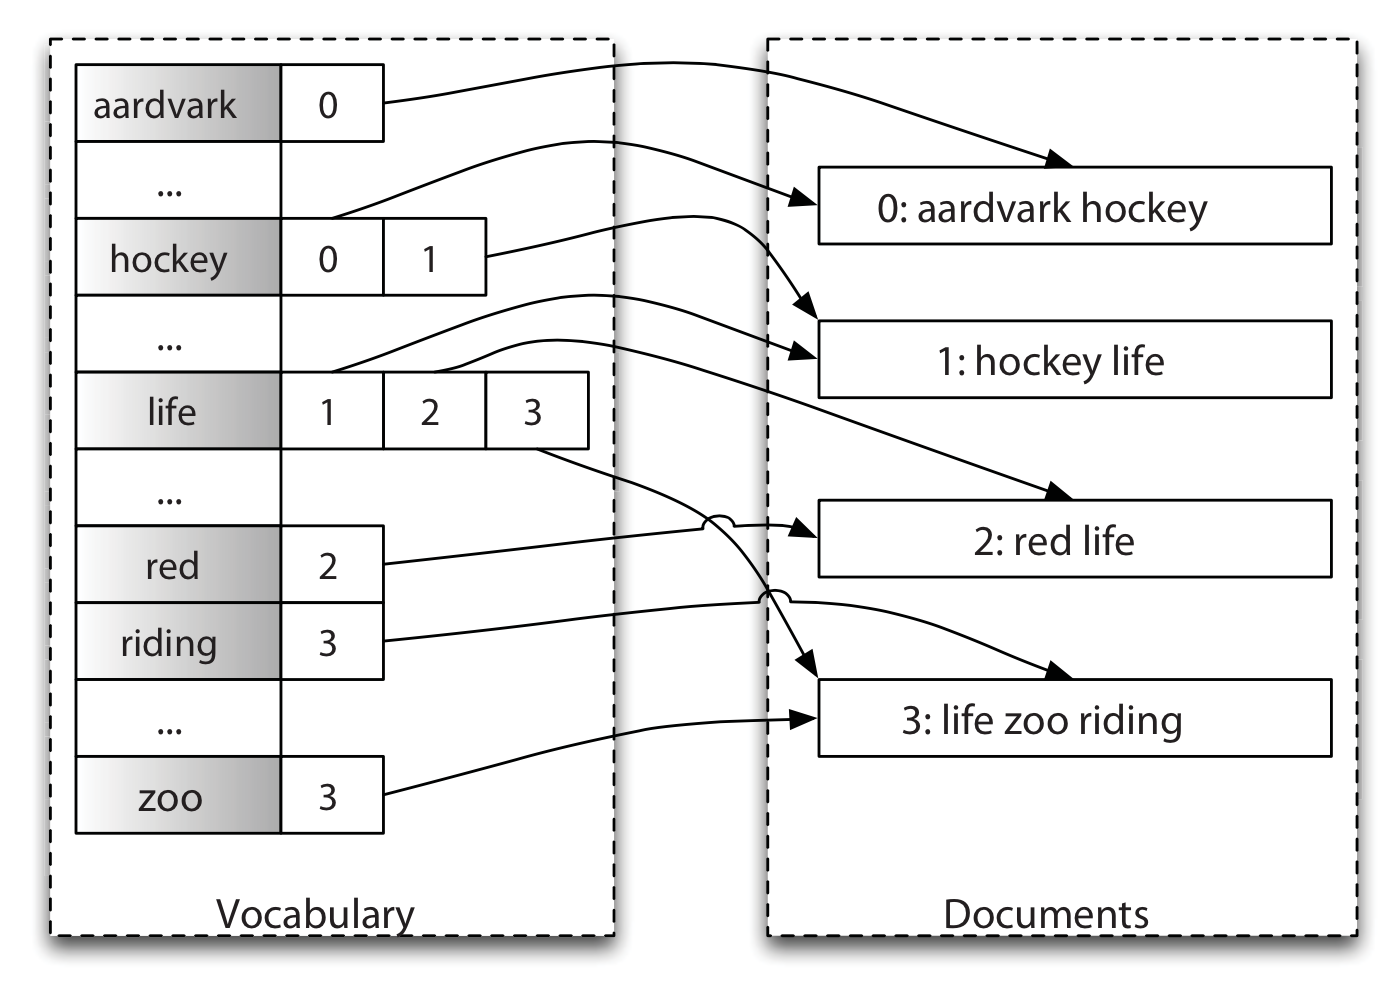
\includegraphics[width=300pt]{inverted_index}
  \caption{Invertirani indeks}
  \label{inverted_index}
\end{figure}

Uz pohranjivanje veza između termova i dokumenata, indeksiranje često uključuje i izračunavanje i spremanje informacija o važnosti termova u odnosu na ostale termove u dokumentu, što je detaljnije objašnjeno u \ref{tfidf}. Ta informacija igra veliku ulogu u omogućavanju tražilice da rangira dokumente po relevantnosti.

\chapter{Upit}

% TODO: Typeahead

Nakon indeksiranja tražilica je spremna za upit. Da bi napravio upit, korisnik komunicira kroz neku vrstu korisničkog sučelja, koje prima jedan ("jednostavno pretraživanje") ili više ("napredno pretraživanje") upita i vraća odgovarajuću listu dokumenata.

Prije nego tražilica počne pretraživati indeks, sam tekst upita obično prolazi isti postupak obrade kao i dokumenti kada se indeksiraju. Primjerice, ako su tokeni korjenovani u indeksu, onda bi i tokeni iz upita također trebali biti korjenovani. U sljedećim sekcijama ćemo navesti dodatne obrade koje tražilica izvršava na samom upitu.

\section{Ključne riječi}

Najosnovniji oblik upita je jednostavno nizanje ključnih riječi odvojenih razmakom (slika \ref{keywords}). Tražilice su obično konfigurirane tako da rezultat takvog upita vrati isključivo dokumente u kojem se nalaze \textit{sve} ključne riječi, da rezultati budu što kvalitetniji. Međutim, ukoliko sama baza aplikacije sadržava vrlo mali broj dokumenata, korisnije je žrtvovati dio kvalitete za kvantitetu, i vratiti sve dokumente koji sadržavaju \textit{bilo koju} od unesenih ključnih riječi.

\begin{figure}[H]
  \centering
  
\includegraphics[width=300pt]{keywords}
  \caption{Primjer upisa ključnih riječi}
  \label{keywords}
\end{figure}

\section{Fraze}

Pretpostavimo da radimo aplikaciju koja omogućuje korisnicima da gledaju riječi pjesama. Pretpostavimo sada da korisnik želi iskoristiti tu aplikaciju da pronađe naziv i autora pjesme na temelju fraza koje je zapamtio iz slušanja te pjesme. Ako korisnik upiše te fraze iz pjesme kao običan niz ključnih riječi, postoji vjerojatnost da će rezultati uključivati i druge pjesme koje sadrže te ključne riječi, i možda pjesma koju korisnik traži neće biti na prvom mjestu. S druge strane, kada bi korisnik mogao reći tražilici da se određeni nizovi riječi iz upita nalaze u dokumentima točno tim redoslijedom, broj vraćenih pjesama se može znatno smanjiti (jer je puno manja vjerojatnost da dvije pjesme dijele čitavu frazu nego par individualnih riječi), i puno je vjerojatnije da će tražena pjesma biti prvi rezultat.

Niz ključnih riječi može se označiti kao fraza tako da se omeđi dvostrukim navodnicima (slika \ref{phrases}). Tražilica pretražuje dokumente za frazu pomoću tzv \textit{n}-grama\footnote{\textit{n}-gram je bilo koji \textit{n}-člani podniz uzastopnih elemenata nekog niza.}. Radi brzine se najprije s manjim \textit{n}-gramima odredi na kojim mjestima je najvjerojatnije da se fraza nalazi, i zatim se ispituju zabilježena mjesta\footnote{\cite{taming} str. 31}.

\begin{figure}[H]
  \centering
  
\includegraphics[width=300pt]{phrases}
  \caption{Primjer upisa fraza}
  \label{phrases}
\end{figure}

\section{Booleovi operatori}

Ranije smo spomenuli da za upit ključnim riječima većina tražilica vraća isključivo dokumente koji sadrže \textit{sve} unešene ključne riječi. Međutim, ako primjerice korisnik koristi online dućan mobilnih telefona, i želi pretražiti sve modele Samsunga i iPhonea, tražilica bi trebala omogućiti korisniku da potraži sve dokumente koji sadrže riječ "iphone" \textit{ili} "samsung".

Zato tražilice obično omogućuju da se između ključnih riječi stave tzv \textit{Booleovi operatori} (slika \ref{boolean}). Operator \textbf{AND} znači da desna i lijeva ključna riječ moraju \textit{obje} biti sadržane u dokumentu, operator \textbf{OR} znači da dokument mora sadržavati \textit{barem jednu} od omeđujućih ključnih riječi, dok operator \textbf{NOT} znači da dokument \textit{ne smije} sadržavati ključnu riječ koja slijedi. Moguće je i korištenje zagrada za gradnju kompleksnijih booleovih izraza.

\begin{figure}[H]
  \centering
  
\includegraphics[width=300pt]{boolean}
  \caption{Primjer booleovih operatora}
  \label{boolean}
\end{figure}

\section{Dodavanje sinonima}

Kada korisnik upiše ključnu riječ "pećina" u polje za pretraživanje, on bi najčešće htio u rezultatima dobiti i dokumente koji sadrže riječ "špilja". Iz tog razloga se često upit proširuje sa sinonimima svake riječi. Na primjer, koristeći booleove operatore, upit "mračna pećina" bi se mogao proširiti na "mračna pećina OR špilja".

Postoji mnogo razloga zašto je dodavanje sinonima bolje raditi na upitu, a ne na indeksu. Proširivanje indeksa sinonimima može znatno povećati indeks, a dodatno je potrebno i reindeksiranje svaki put kada se lista sinonima ažurira.

\section{Zamjenski znakovi i regularni izrazi}

Naprednijim korisnicima trebalo bi omogućiti maksimalnu preciznost pretraživanja. U tu svrhu može se omogućiti upotreba zamjenskih znakova \textit{?}, koji reprezentira 1 proizvoljan znak, i \textit{*}, koji reprezentira bilo koji broj (uključujući i 0) proizvoljnih znakova (slika \ref{wildcards}). Tako će \textit{bank?} pronaći riječi "banka", "banke", "banki" itd, dok će \textit{bank*} pronaći i riječi kao "bankama" i "bankarstvo".

\begin{figure}[H]
  \centering
  
\includegraphics[width=300pt]{wildcards}
  \caption{Primjer zamjenskih znakova}
  \label{wildcards}
\end{figure}

Dok su ova 2 zamjenska znakova daju kontrolu dovoljnu u većini slučajeva, postoje rijetki slučajevi u kojima je potrebna veća preciznost (npr. pretraživanje programskog kôda). Zato neke tražilice omogućuju i korištenje regularnih izraza\footnote{\url{http://en.wikipedia.org/wiki/Regular_expression}} u upitu.

\section{Ispravljanje zatipaka}

Pri unosu upita, često se mogu pojaviti zatipci (eng. \textit{typographical error}); bilo zato što korisnik ne zna kako se neka riječ piše (npr. ako piše na engleskom), ili je korisnik jednostavno pritisnuo krivu tipku na tastaturi, i nije to primjetio. Štoviše, zatipci se mogu pojaviti i u tekstu koji se pretražuje.

Zato je uobičajeno da tražilica tolerira određeni stupanj "greške" u unosu. Ukoliko tražilica ne pronađe danu riječ u indeksu, ona pokuša pronaći dokumente sa riječima koje su "slične" riječi iz upita. Neke tražilice čak idu dalje i u slučaju velike sigurnosti ponude korisniku ispravljenu riječ.

Spomenuli smo pojam međusobne "sličnosti" riječi, ali nismo definirali kako se to izračunava. Ovdje je opet od velike pomoći promatranje \textit{n}-grama. Ranije smo radili s \textit{n}-gramima na razini riječi, ali ovaj puta promatramo \textit{n}-grame na razini slova. Najbolja mjera za sličnost dviju riječi je broj zajedničkih \textit{n}-grama\footnote{\cite{taming} str. 99}, konkretnije trigrama\footnote{\url{http://www.postgresql.org/docs/9.4/static/pgtrgm.html}}.

\section{Automatsko nadopunjavanje}

Dok korisnik upisuje znakove u polje za upit, aplikacije često otvaraju listu sugestija iz dokumenata koji se nalaze u indeksu, na temelju znakova koje je korisnik trenutno upisao (slika \ref{typeahead}). (Najčešće se taj niz znakova uzima kao prefix.) To poboljšava korisničko iskustvo na više načina. Prvo, korisniku može skratiti količinu tipkanja tako da korisnik izabere sugestiju umjesto da završi tipkati. Drugo, ako korisnik dobije listu sugestija, onda zna da do sada nije napravio prevelike zatipke. Treće, automatska povratna informacija o korisnikovim upisanim znakovima vodi korisnika da napravi upit koji će sigurno vratiti rezultate.

\begin{figure}[H]
  \centering
  
\includegraphics[width=300pt]{typeahead}
  \caption{Primjer automatskog nadopunjavanja na \url{www.google.com}}
  \label{typeahead}
\end{figure}

Lista sugestija se najčešće dobavlja korištenjem \textit{n}-grama, na sličan način kao kod ispravljanja zatipaka. Najprije se dobavljaju riječi koje sadrže barem jedan zajednički \textit{n}-gram s upitom, a zatim se ta lista rangira po broju zajedničkih \textit{n}-grama\footnote{\cite{taming} str. 100}.

\section{Kategorizacija}

Pretpostavimo da korisnik želi kupiti čvrsti disk, ali ne zna točno koji želi. Korisnik otvori \url{www.nabava.net}, i uđe u kategoriju "Računala > Pohrana podataka > Čvrsti diskovi" (slika \ref{nabava1}).

\begin{figure}[H]
  \centering
  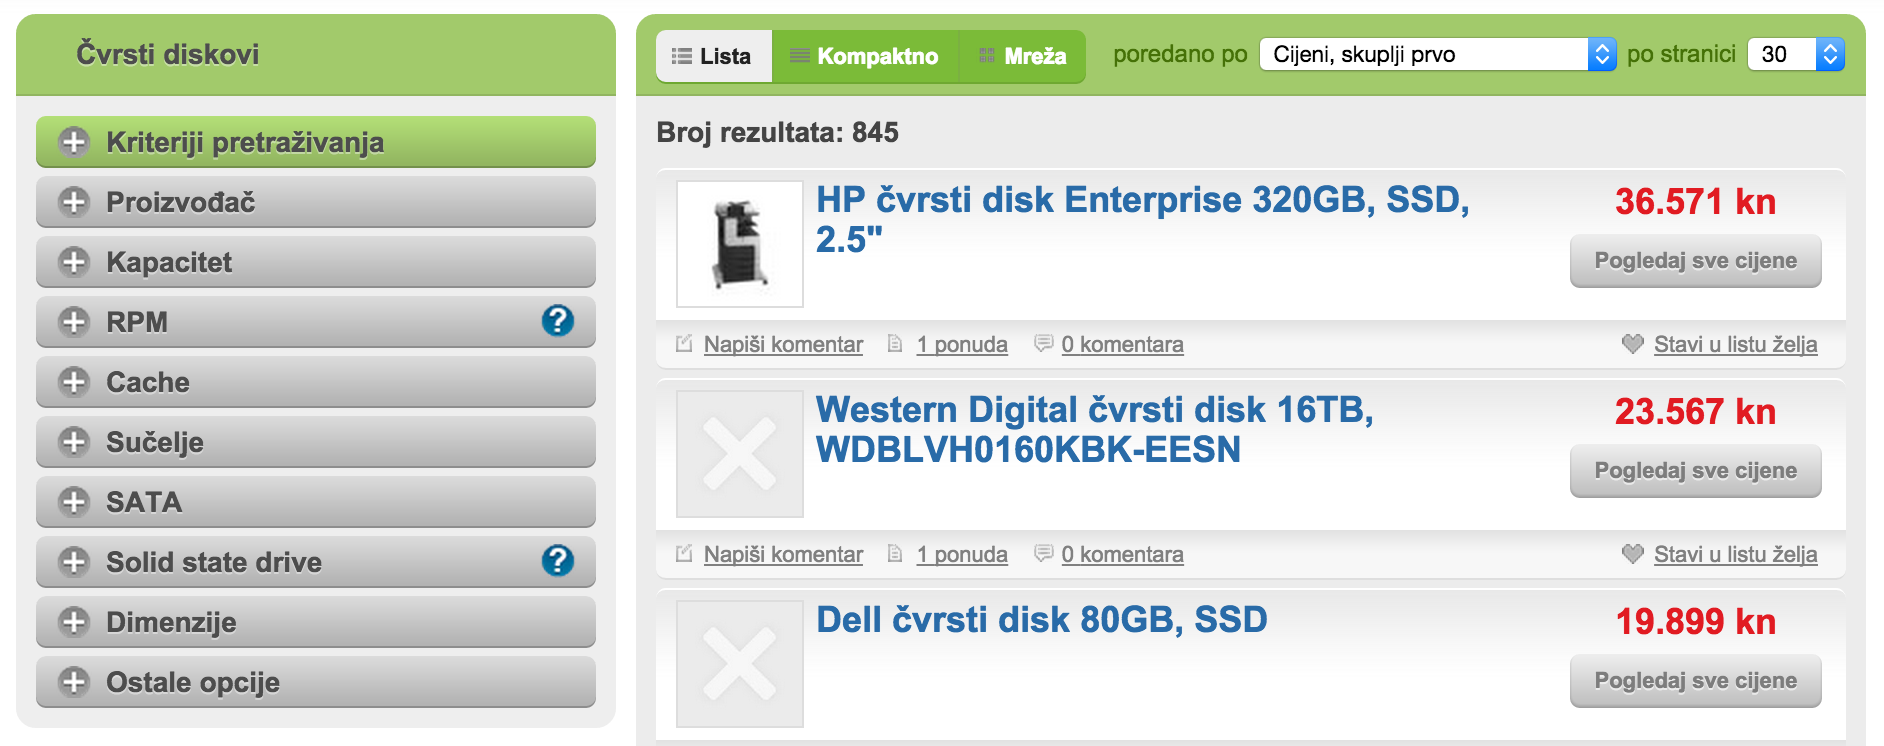
\includegraphics[width=\textwidth]{nabava1}
  \caption{Kategorija "Čvrsti diskovi" na \url{www.nabava.net}}
  \label{nabava1}
\end{figure}

Korisnik zatim počne razmišljati koji točno čvrsti disk želi. Čuo je da kompanija HP proizvodi dobre čvrste diskove, i u lijevom izborniku označi da želi sve čvrste diskove od te kompanije (slika \ref{nabava2}).

\begin{figure}[H]
  \centering
  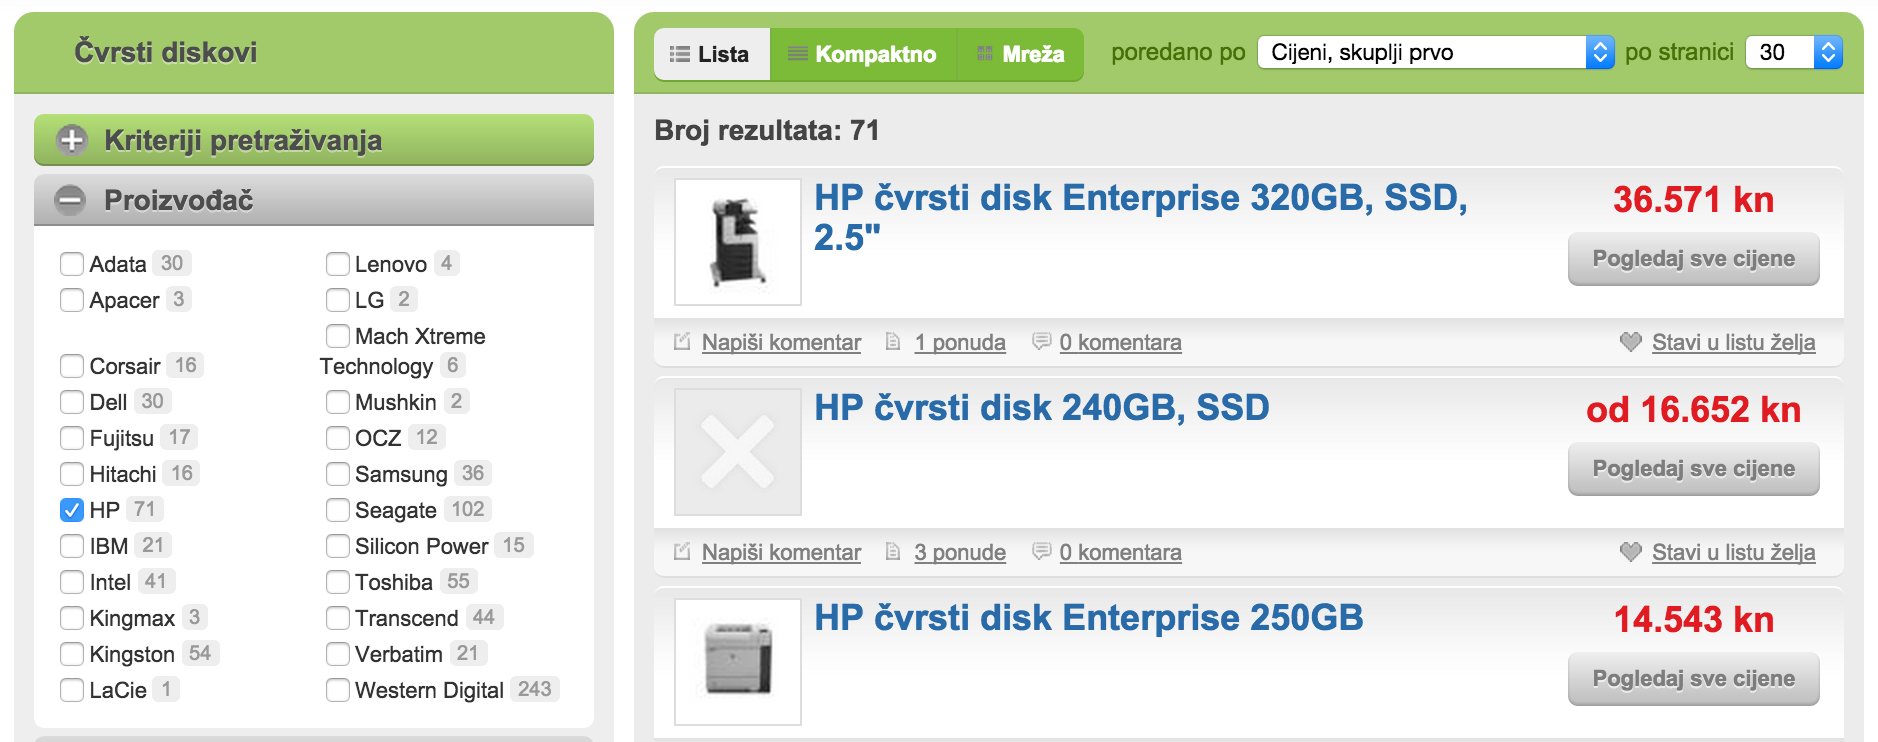
\includegraphics[width=\textwidth]{nabava2}
  \caption{Filtriranje kompanije na \url{www.nabava.net}}
  \label{nabava2}
\end{figure}

Budući da korisnik želi na taj disk uglavnom spremati filmove, odluči da mu treba disk s većim kapacitetom, te u lijevom izborniku označi kapacitet "512GB - 2TB" (slika \ref{nabava3}).

\begin{figure}[H]
  \centering
  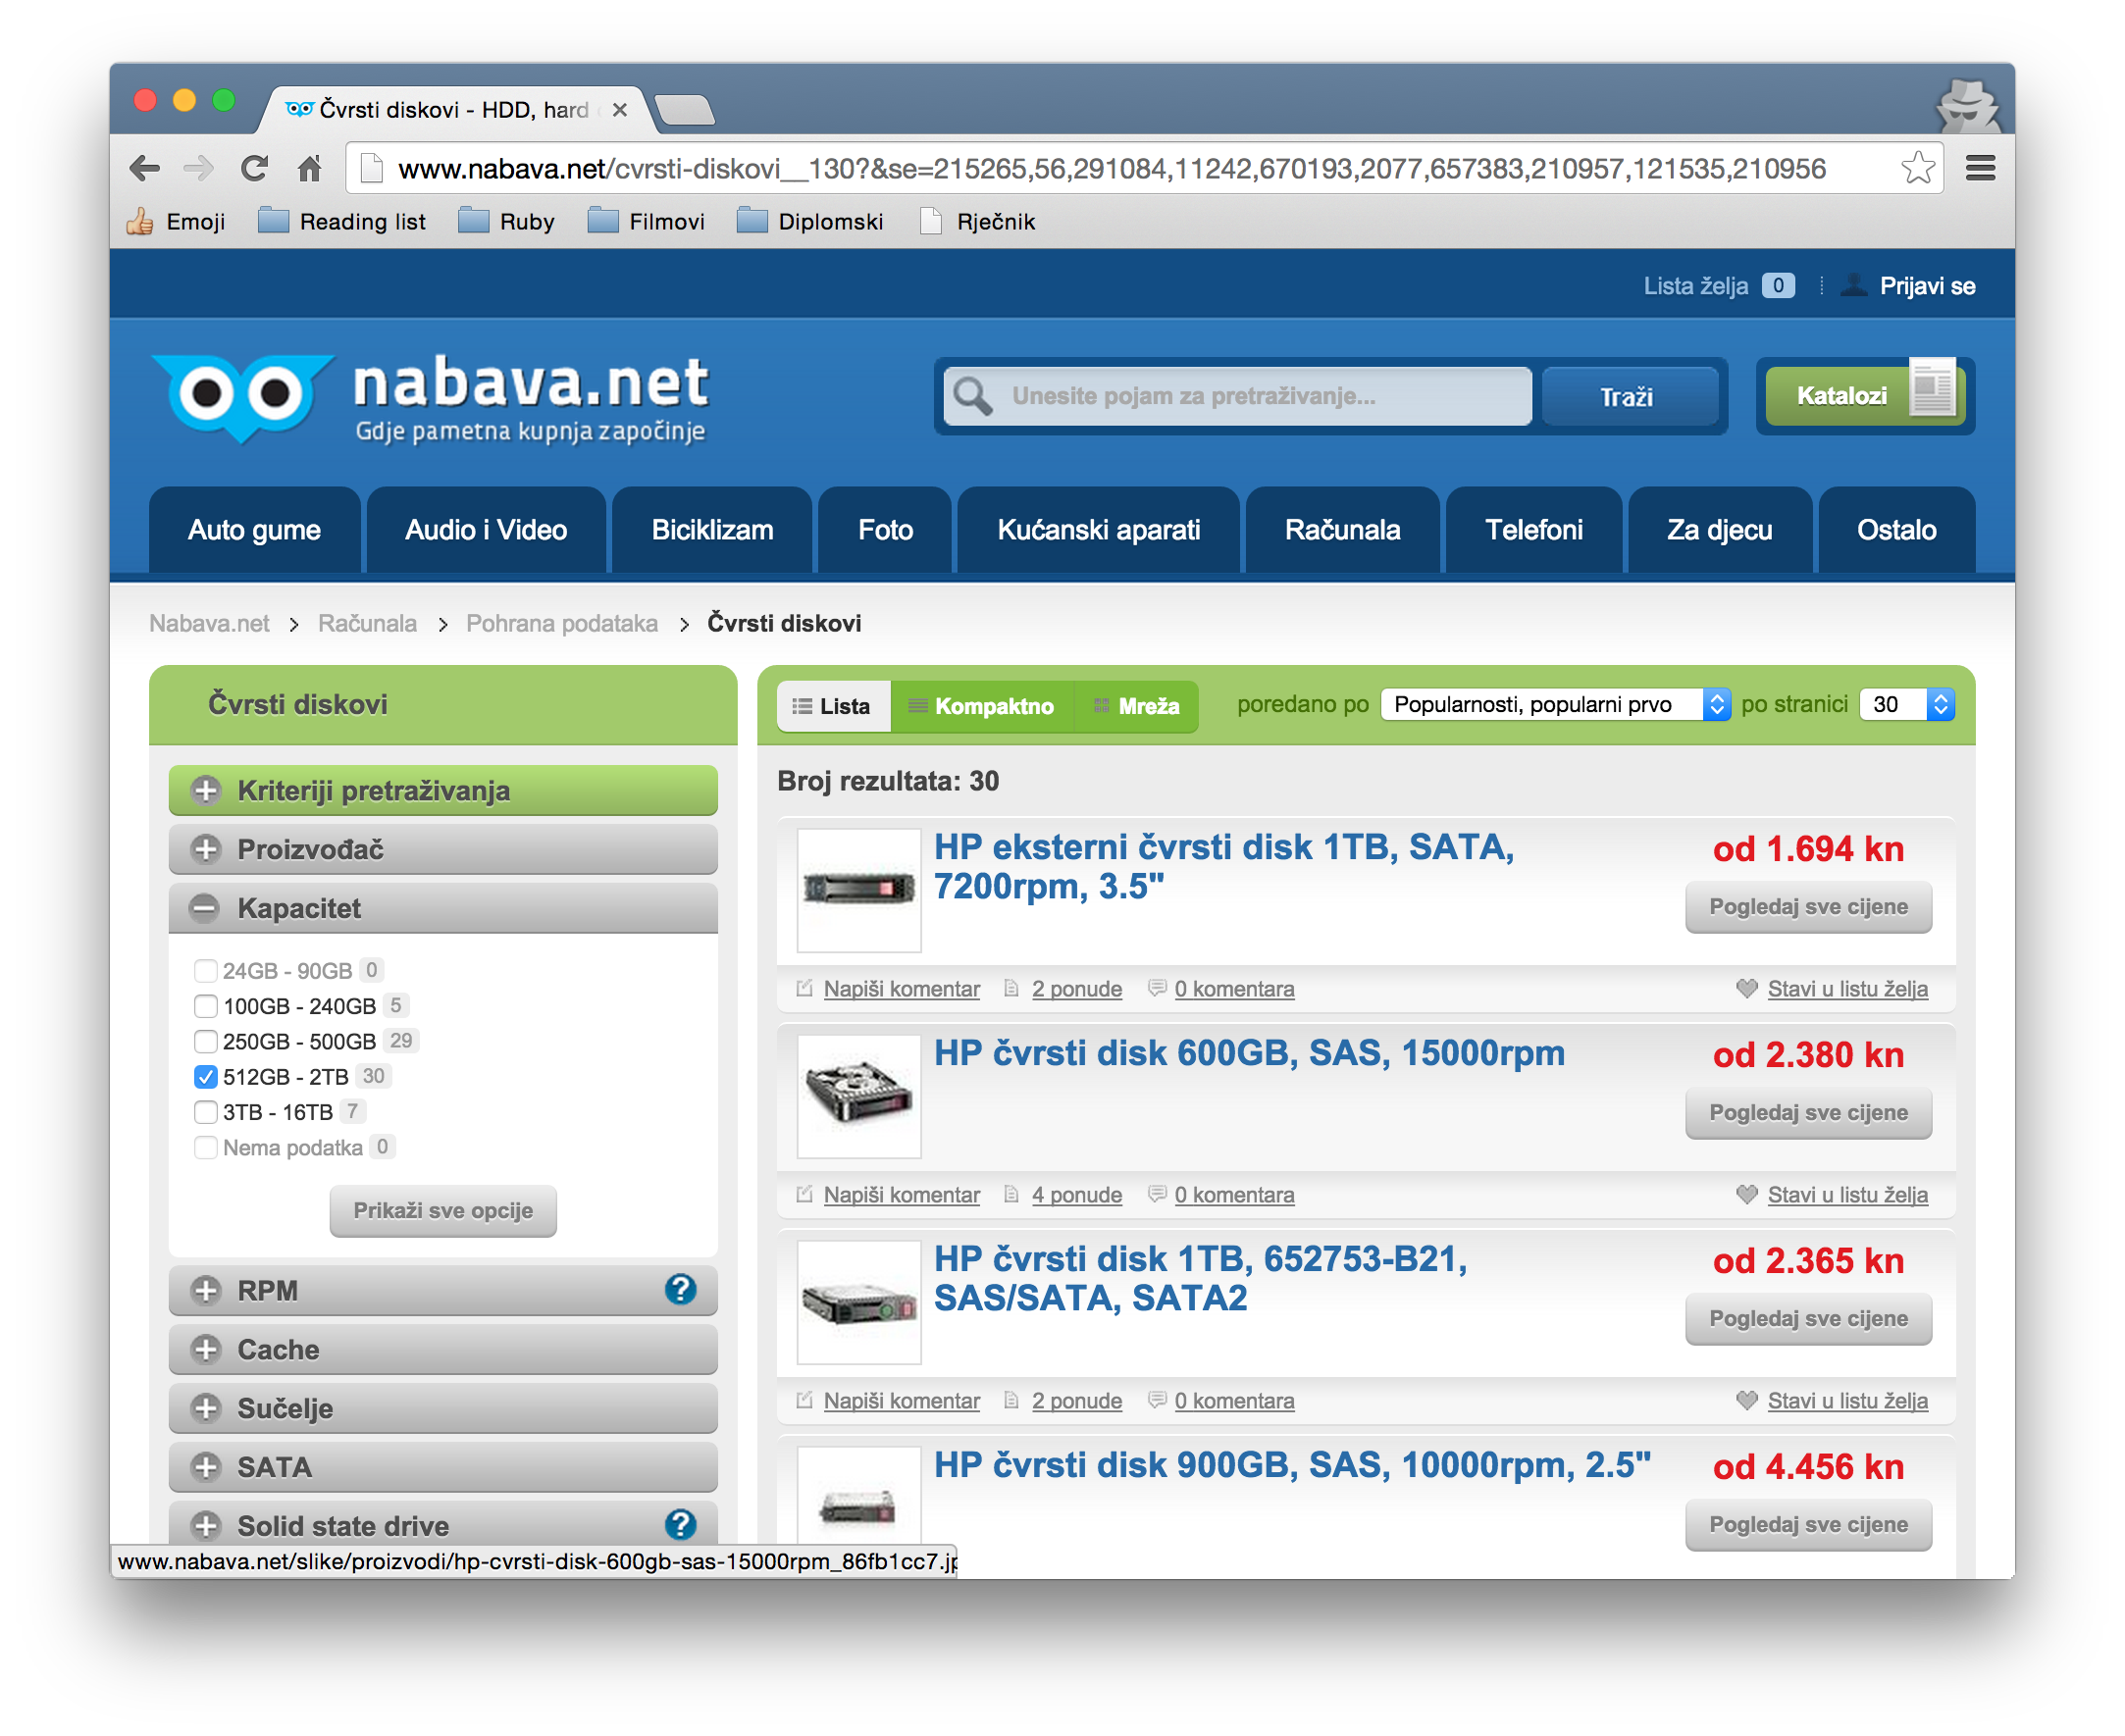
\includegraphics[width=\textwidth]{nabava3}
  \caption{Filtriranje kapaciteta diska na \url{www.nabava.net}}
  \label{nabava3}
\end{figure}

I uz odgovarajuće sortiranje korisnik pronađe željeni disk. Da korisnik nije imao lijevi izbornik koji mu je pomogao filtrirati proizvode po određenim kategorijama, teško bi mogao naći željeni čvrsti disk, jer u ovim slučajevima jedno tekstualno polje za pretraživanje nije dovoljno.

Dok se pretraživanje po ključnim riječima koristi kada korisnik zna što želi naći i samo želi doći do toga u aplikaciji, kategorizacija (eng. \textit{faceting}) je vrlo korisna kada korisnik ne zna točno što traži, nego želi vidjeti što je "dostupno". Kod pretraživanja po ključnim riječima korisnik očekuje željeni dokument u prvih par rezultata, dok kategorizacija ne treba pružati tu garanciju, jer su kategorije često vrlo generičke.

Tražilice obično imaju mogućnost vratiti listu dostupnih kategorija (izvađenih iz metapodataka dokumenta), i broj dokumenata koje svaka kategorija sadrži. Garantirano je da svaka vraćena kategorija sadrži barem jedan dokument.

\section{Paginacija}

Ukoliko je indeks jako velik, traženje \textit{svih} dokumenata koji odgovaraju nekom upitu može trajati dugo. Također, aplikacije najčešće ne žele prikazati sve rezultate na stranici odjednom, jer bi stranica bila prevelika.

Iz tog razloga tražilice često uz upit prihvaćaju i opciju (a) koliko dokumenata tražilica treba vratiti (eng. \textit{limit}) i (b) koji prozor rezultata treba vratiti (eng. \textit{offset}). Na taj način aplikacija primjerice može implementirati paginaciju (slika \ref{pagination}).

\begin{figure}[H]
  \centering
  
\includegraphics[width=300pt]{pagination}
  \caption{Paginacija na \url{www.nabava.net}}
  \label{pagination}
\end{figure}

Paginacija je moguća i efektivna jer se rangiranje odvija pri pretraživanju, na način da se prvo pretražuju dokumenti koji izgledaju "relevantnije". Nakon što se pronašao tražen broj dokumenata, pretraga može stati.

\chapter{Rangiranje}

Dok tražilica pretražuje sve dokumente koji odgovaraju danom upitu, potrebno je odrediti koliko je neki dokument "relevantan" upitu. Iako je tražilicama obično moguće proslijediti opciju sortiranja rezultata po nekom kriteriju (npr. alfabetično ili po cijeni), odsustvo te opcije podrazumijeva da tražilica vraća rezultate sortirane po "relevantnosti".

\section{Model vektorskog polja}

Da bismo rangirali dokumente, potrebno je definirati mjeru "relevantnosti" upitu. Najprije je potrebno postaviti model u kojem ćemo definirati tu mjeru. Postoji mnogo različitih modela, a mi ćemo promatrati najpopularniji – model vektorskog polja.

Ideja modela vektorskog polja je promatranje dokumenata kao vektore u \textit{n}-dimenzionalnom vektorskom prostoru. Vektorski prostor je definiran tako da svaka dimenzija odgovara jednom tokenu iz skupa svih jedinstvenih tokena iz svih dokumenata. Na primjer, pretpostavimo da imamo kolekciju sljedećih dokumentata:

\begin{compactenum}
  \item "Ivica Kostelić odnosi pobjedu u skijaškom kupu"
  \item "Janica Kostelić odnosi pobjedu u svjetskom prvenstvu"
\end{compactenum}

Tada modeliramo ova dva dokumenta kao vektore u $10$-dimenzionalnom vektorskom prostoru (budući da unija tokena iz gornja dva dokumenta čini $10$-člani skup). Budući da su dokumenti zapravo niz tokena, možemo ih promatrati kao vektore u tom vektorskom prostoru kojemu je dimenzija \textit{k} jednaka $1$, ako token \textit{k} postoji u dokumentu, ili $0$, ako token ne postoji u dokumentu. Neka numeriramo tokene iz našeg primjera na sljedeći način:

\begin{center}
  \begin{tabular}{@{\enspace}c@{\enspace}c@{\enspace}c@{\enspace}c@{\enspace}c@{\enspace}c@{\enspace}c@{\enspace}c@{\enspace}c@{\enspace}c@{\enspace}}
    1     & 2      & 3        & 4      & 5       & 6 & 7         & 8         & 9    & 10        \\
    ivica & janica & kostelić & odnosi & pobjedu & u & skijaškom & svjetskom & kupu & prvenstvu \\
  \end{tabular}
\end{center}

Tada naša dva dokumenta postaju sljedeći vektori:

\begin{compactenum}
  \item $(1,0,1,1,1,1,1,0,1,0)$
  \item $(0,1,1,1,1,1,0,1,0,1)$
\end{compactenum}

Sada kada smo definirali model vektorskog polja, možemo definirati pojam "relevantnosti" dokumenta upitu. Ukoliko gledamo i upit kao vektor u istom vektorskom prostoru, možemo promatrati koliko se upit podudara s dokumentom tako gledamo kut između ta dva vektora. Ukoliko je kut $0\degree$, znači da imamo potputno podudaranje. Onda možemo definirati "relevantnost" kao kosinus tog kuta, koji će uvijek biti broj između $-1$ i $1$, s time da će biti maksimalan ($1$) upravo kada je kut $0\degree$.

\section{Težina riječi} \label{tfidf}

Da bi se poboljšala kvaliteta tražilice, umjesto samo spremanja $1$ za indikaciju da riječ postoji u dokumentu, tražilice obično spremaju neku vrstu težine koja predstavlja relativnu važnost te riječi u odnosu na ostale riječi.

Najčešći sustav težina koji se koristi je \textit{TF-IDF} (eng. \textit{Term Frequency – Inverse Document Frequency}). Glavna ideja je sljedeća; riječ koja se pojavljuje često u dokumentu je važnija, osim ako se pojavljuje često i u ostalim dokumentima. Drugim riječima, važnost riječi je proprocionalna broju pojavljivanja u dokumentu (TF) i obrnuto proporcionalna općenitom broju pojavljivanja u svim dokumentima (IDF).

U našem primjeru, u prvom dokumentu se riječ "Ivica" pojavljuje $1$ puta, dok se u drugom dokumentu ne pojavljuje. Dakle njena prosječna frekvencija je $0.5$, iz čega slijedi da je njena težina $TF / IDF = 1 / 0.5 = 2$. S druge strane, riječ "u" se u oba dokumenta pojavljuje 1 puta, pa je njena težina $1 / 1 = 1$. Napravimo li to za svaku riječ, prvi dokument postaje $$(2,0,1,1,1,1,2,0,2,0)$$

\section{Blizina riječi}

Kod rangiranja je također korisno promatrati koliko su pronađene ključne riječi međusobno udaljene. Kada su pronađene ključne riječi međusobno bliže, onda je dokument intuitivno relevantniji, zato tražilice najčešće rangiraju takve dokumente više. Specijalno, ako su pronađene ključne riječi u dokumentu uzastopne, odnosno ako tvore frazu, taj će se dokument će dobiti veću relevantnost. To znači da, ako je npr. upit jednak naslovu dokumenta, taj dokument će se vrlo vjerojatno rangirati prvi, što odgovara korisnikovim očekivanjima.

\section{Težina dijelova dokumenata}

Kao što je spomenuto u poglavlju \ref{indexing}, dokumenti su često indeksirani u dijelovima kojima je dana različita težina. Na primjer, ako se radi o vijestima za novine, naslov vijesti će najčešće imati veću težinu nego sam sadržaj. Zato se dokumenti rangiraju drukčije s obzirom na to koji dio upita se podudara s kojim dijelom dokumenta.

\chapter{Implementacija}

\section{Softveri}

\subsection{Apache Solr}

\subsection{Sphinx}

\subsection{PostgreSQL}

\subsection{ElasticSearch}

\section{Aplikacija}

\chapter{Rezultati}

\chapter{Zaključak}

% TODO: Cross-language searching

\section{Poboljšavanje performansi}

% TODO: 3.6 & 3.7

\begin{thebibliography}{99}
  \bibitem{taming} G. S. Ingersoll, T. S. Morton, A. L. Farris, \textit{Taming Text: How to Find, Organize, and Manipulate It}, Manning Publications Co, Zagreb, 2013.
  \bibitem{elastic} C. Gormley, Z. Tong, dostupno na \url{http://www.elasticsearch.org/guide/en/elasticsearch/guide/current/index.html} (veljača 2014.)
\end{thebibliography}

\pagestyle{empty}

\begin{sazetak}
\end{sazetak}

\begin{summary}
\end{summary}

\begin{cv}
\end{cv}

\end{document}
